\subsubsection{Listar}

  \paragraph{}Para mostrar esta lista, es necesario establecer el asesor para
  el que mostrar las preguntas de reunión disponibles. Para ello, habrá que
  elegir el asesor en la lista desplegable que se muestra en la figura
  \ref{capturaPantallaSelectAsesor}.

  \paragraph{}También habrá que seleccionar el curso académico para el que
  listar las preguntas de reunión del asesor seleccionado. La figura
  \ref{capturaPantallaSelectAsesorCursoAcademico} muestra una captura de
  pantalla de la lista desplegable para seleccionarlo.

  \paragraph{}Además, habrá que elegir el alumno para el que mostrar las
  preguntas de reunión existentes. Para ello, se seleccionará en una lista
  desplegable, tal y como muestra la captura de pantalla de la figura
  \ref{capturaPantallaSelectAlumno}.

  \paragraph{}Por último, es necesario seleccionar la reunión para la que se
  mostrarán las preguntas de reunión. Es posible ver una captura de pantalla
  de esta ventana en la figura \ref{capturaPantallaSelectReunion}.

  \paragraph{}Nótese que si no existieran elementos disponibles en el sistema,
  la lista desplegable aparecería vacía. Por tanto, se proporciona al usuario
  un icono, representado por una cruz verde, para añadir nuevos elementos al
  sistema. Este icono es el mostrado en la figura \ref{capturaBotonAdd}. Al
  pulsar dicho botón, aparecerá la ventana de creación de un nuevo elemento.

  \paragraph{}Una vez seleccionado el asesor entre los disponibles, se muestra
  la lista completa de preguntas de asesor para la reunión que aparecen en el
  sistema. La figura
  \ref{capturaPantallaListaPreguntasOficialesReunionAdminPrincipal} muestra una
  captura de pantalla de la lista de preguntas de asesor de la reunión.

  \begin{figure}[!ht]
    \begin{center}
      \fbox{
      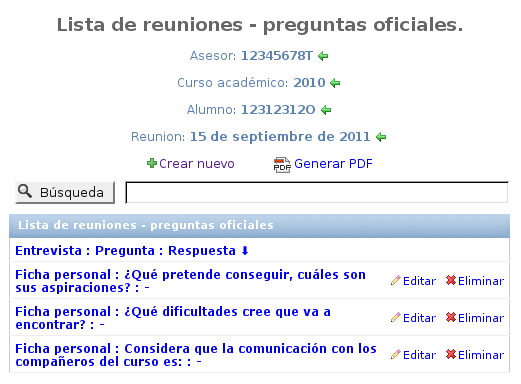
\includegraphics[scale=0.55]{4.Funcionamiento_Aplicacion/4.3.Gestion/4.3.1.Administrador_Principal/4.3.1.17.Reunion_PreguntaOficial/lista_preguntasOficiales_reunion.png}
      }
      \caption{Captura de pantalla de la lista de preguntas oficiales para una reunión para el usuario \textit{Administrador principal}.}
      \label{capturaPantallaListaPreguntasOficialesReunionAdminPrincipal}
    \end{center}
  \end{figure}
